\documentclass[a4paper,norsk, 10pt]{article}
\usepackage[utf8]{inputenc}
\usepackage{verbatim}
\usepackage{listings}
\usepackage{graphicx}
\usepackage[norsk]{babel}
\usepackage{a4wide}
\usepackage{color}
\usepackage{amsmath}
\usepackage{float}
\usepackage{amssymb}
\usepackage[dvips]{epsfig}
\usepackage[toc,page]{appendix}
\usepackage[T1]{fontenc}
\usepackage{cite} % [2,3,4] --> [2--4]
\usepackage{shadow}
\usepackage{hyperref}
\usepackage{titling}
\usepackage{marvosym }
\usepackage{subcaption}
\usepackage[noabbrev]{cleveref}
\usepackage{cite}


\setlength{\droptitle}{-10em}   % This is your set screw

\setcounter{tocdepth}{2}

\lstset{language=c++}
\lstset{alsolanguage=[90]Fortran}
\lstset{alsolanguage=Python}
\lstset{basicstyle=\small}
\lstset{backgroundcolor=\color{white}}
\lstset{frame=single}
\lstset{stringstyle=\ttfamily}
\lstset{keywordstyle=\color{red}\bfseries}
\lstset{commentstyle=\itshape\color{blue}}
\lstset{showspaces=false}
\lstset{showstringspaces=false}
\lstset{showtabs=false}
\lstset{breaklines}
\title{FYS3120 Oblig 5}
\author{Daniel Heinesen, daniehei}
\begin{document}
\maketitle
\section*{1)}
\subsection*{a)}
The given coordinates for a rotating frame are 

$$
x = \xi\cos\omega t - \eta\sin\omega t
$$
$$
y = \xi\sin\omega t + \eta\cos\omega t
$$

To find the Lagrangian we are going to start with the

$$
\dot{x} = -\xi\omega\sin\omega t - \eta\omega\cos\omega t + \dot{\xi}\cos\omega t - \dot{\eta}\sin\omega t
$$
$$
\dot{y} = \xi\omega\cos\omega t - \eta\omega\sin\omega t + \dot{\xi}\sin\omega t + \dot{\eta}\cos\omega t
$$

The energies of the system is as follows

$$
V = mgy = mg(\xi\sin\omega t + \eta\cos\omega t)
$$
$$
T = \frac{1}{2}m(\dot{x}^2 + \dot{y}^2) = \frac{1}{2}m(\xi^2\omega^2 + \eta^2\omega^2 + 2\xi\dot{\eta}\omega - 2\eta\dot{\xi}\omega + \dot{\xi}^2 + \dot{\eta}^2)
$$

Giving us the Lagrangian

$$
L = \frac{1}{2}m(\xi^2\omega^2 + \eta^2\omega^2 + 2\xi\dot{\eta}\omega - 2\eta\dot{\xi}\omega + \dot{\xi}^2 + \dot{\eta}^2)- mg(\xi\sin\omega t + \eta\cos\omega t)
$$

\subsection*{b)}
We can now find the corresponding e.o.m's

$$
\frac{\partial L}{\partial \xi} = m(\xi \omega^2 + \dot{\eta}\omega) - mg\xi\sin\omega t
$$
$$
\frac{\partial L}{\partial \dot{\xi}} = m(\dot{\xi} - \eta\omega)
$$
$$
\frac{d}{dt}\left(\frac{\partial L}{\partial \dot{\xi}}\right) = m(\ddot{\xi} - \dot{\eta}\omega)
$$

Giving us the first e.o.m

\begin{equation}
m\ddot{\xi} - 2m\dot{\eta}\omega - m\omega^2\xi+ mg\xi\sin\omega t = 0
\label{eq:xieom}
\end{equation}

For the second e.o.m

$$
\frac{\partial L}{\partial \eta} = m(\eta\omega^2 - \dot{\xi}\omega) - mg\eta \cos\omega t
$$
$$
\frac{\partial L}{\partial \dot{\eta}} = m(\dot{\eta} + \xi\omega)
$$
$$
\frac{d}{dt}\left(\frac{\partial L}{\partial \dot{\eta}}\right) =  m(\ddot{\eta} + \dot{\xi}\omega)
$$

Giving us the second e.o.m

\begin{equation}
m\ddot{\eta} + 2m\dot{\xi}\omega -m\omega^2\eta + mg\eta \cos\omega t = 0
\label{eq:etaeom}
\end{equation}

We can combine these and get that 

\begin{equation}
m(\ddot{\eta} + \ddot{\xi}) - 2m\omega(\dot{\eta} -\dot{\xi}) - m\omega^2(\eta + \xi) + mg(\eta\cos\omega t + \xi\sin\omega t) = 0
\label{eq:eom}
\end{equation}

From both the e.o.m we can see that there are terms corresponding to the Coriolis- and the centrifugal force. In a general physics book the Coriolis force is given as $-2m\vec{\Omega}\times \vec{v}$, which we can recognize from our e.o.m as $- 2m\omega(\dot{\xi} -\dot{\eta}) $.\\

Centripetal force is generally given as $-m\vec{\Omega}\times(\vec{\Omega}\times \vec{r})$ which we recognize as $- m\omega^2(-\eta - \xi)$ \\

For a rotating frame, Newton's 2nd law is given as

$$
ma = F_{imp} + F_{centrifugal} + F_{Coriolis}
$$

We see that this has the exact same form as our e.o.m \ref{eq:eom}

$$
\underbrace{m(\ddot{\eta} + \ddot{\xi})}_{ma} = \underbrace{2m\omega(\dot{\xi} -\dot{\eta})}_{F_{Coriolis}} + \underbrace{m\omega^2(-\eta - \xi)}_{F_{centrifugal}} + \underbrace{mg(\eta\cos\omega t + \xi\sin\omega t)}_{F_{imp}}
$$




\section*{2)}
\subsection*{a)}
We want to find the time it takes to get between A and B. We are going to start with our old friend

$$
s = vt
$$

We are the going to do this for infinitesimals

$$
ds = v dt 
$$

We know that 

$$
ds = \sqrt{dx^2 + dy^2} =\sqrt{1 + \left(\frac{dy}{dx}\right)^2}dx= \sqrt{1 +y'^2} dx
$$

We then need to find $v$. We know that energy is conserved, so

$$
\frac{1}{2}mv^2 + mgy = 0 \Rightarrow v = \sqrt{-2gy}
$$

Given that $y>0$\\
We can now combine these 3 facts, and we get that

$$
dt = \frac{ds}{v} = \sqrt{\frac{1 + y'^2}{-2gy}}dx
$$

We can now find the total time

$$
T[y(x)] = \int dt = \int_{x_A}^{x_B} \sqrt{\frac{1 + y'^2}{-2gy}}dx = \int_{x_A}^{x_B} L(y,y') dx
$$




\subsection*{b)}
The Hamiltonian $H$ is given by

$$
H = py' - L
$$

Since $L$ has no explicit time-dependence, the Hamiltonian is a constant of motion, $E$.\\

To calculate the Hamiltonian we start by calculating

$$
p = \frac{\partial L}{\partial y'} = \frac{y'}{-2gy}\sqrt{\frac{2gy}{1+y'^2}}
$$

And then we get

$$
H = \frac{y'^2}{-2gy}\sqrt{\frac{2gy}{1+y'^2}} - \sqrt{\frac{1 + y'^2}{-2gy}} = E
$$

Dividing the whole expression by $\sqrt{\frac{2gy}{1+y'^2}}$ we get

$$
\frac{1}{-2gy}y'^2 - \frac{1+y'^2}{-2gy} = E \sqrt{\frac{1 + y'^2}{-2gy}}
$$

Cleaning up some, and then squaring both sides gives us

$$
\left(\frac{1}{-2gy}\right)^2 = E^2\frac{1+y'^2}{-2gy}
$$

$$
\Rightarrow \frac{1}{-2gy} = E^2(1+y'^2)
$$

This gives us the differential equation

\begin{equation}
(1+y'^2)y = \frac{1}{-2gE^2} = -k^2
\label{eq:diff}
\end{equation}

\subsection*{c)}

We are given 

\begin{equation}
x = \frac{1}{2}k^2(\theta - \sin\theta)
\label{eq:x}
\end{equation}
\begin{equation}
y = \frac{1}{2}k^2(\cos\theta - 1)
\label{eq:y}
\end{equation}

We need to find $y'$, for this we need

\begin{equation}
\frac{dx}{d\theta} = \frac{1}{2}k^2(1-\cos\theta)
\label{eq:dxdt}
\end{equation}

\begin{equation}
\frac{dy}{d\theta} = -\frac{1}{2}k^2\sin\theta
\label{eq:dydt}
\end{equation}

Combining them gives us

\begin{equation}
\frac{dy}{dx} = \frac{\sin\theta}{\cos\theta - 1}
\label{eq:dydx}
\end{equation}

We now insert this into \ref{eq:diff}

$$
(1+y'^2)y = (1+\left(\frac{\sin\theta}{\cos\theta - 1}\right)^2)\frac{1}{2}k^2(\cos\theta - 1)
$$
$$
= \frac{1}{2}k^2(\cos\theta -1) + \frac{1}{2}k^2\frac{\sin^2\theta}{\cos\theta - 1} = \frac{1}{2}k^2\left[\frac{(\cos\theta -1)^2 + \sin^2\theta}{\cos\theta - 1}\right]
$$

$$
= \frac{1}{2}k^2\left[\frac{2 - 2\cos\theta}{\cos\theta - 1}\right] = -k^2
$$

This shows that \ref{eq:x} and \ref{eq:y} solves the differential equation \ref{eq:diff}.\\

If we have boundary conditions $(x_A,y_A)$ and $(x_B,y_B)$ we need to find the corresponding pair $(r,\theta)$ for both points, where $r = \frac{1}{2}k^2$ is constant for both points. We are going to assume for the sake of discussion that the point A is at the origin, so that $\theta_A = 0$. We can then find $\theta_B$ by solving

$$
\frac{x_B}{y_B} = \frac{\theta_B - \sin\theta_B}{\cos\theta_B - 1}
$$

This is difficult to solve analytically for $\theta_B$, but easy numerically.\\

We can use $\theta_ B$ to find $r$

$$
x_B = r(\theta_B - \sin\theta_B) \Rightarrow r = \frac{x_B}{(\theta_B - \sin\theta_B)}
$$

If we now let $\theta \in [0,\theta_B]$ and $\frac{1}{2}k^2 = r$ we get a brachistochrone from $(0,0)$ to $(x_B,y_B)$. If we want to use another starting point we just need to calculate a new $\theta_A$, and move the all the y-coordinates by $y_A$(Since \ref{eq:x} and \ref{eq:y} always has it origin at $(0,0)$)

\subsection*{d)}
\begin{figure}[H]
\centering
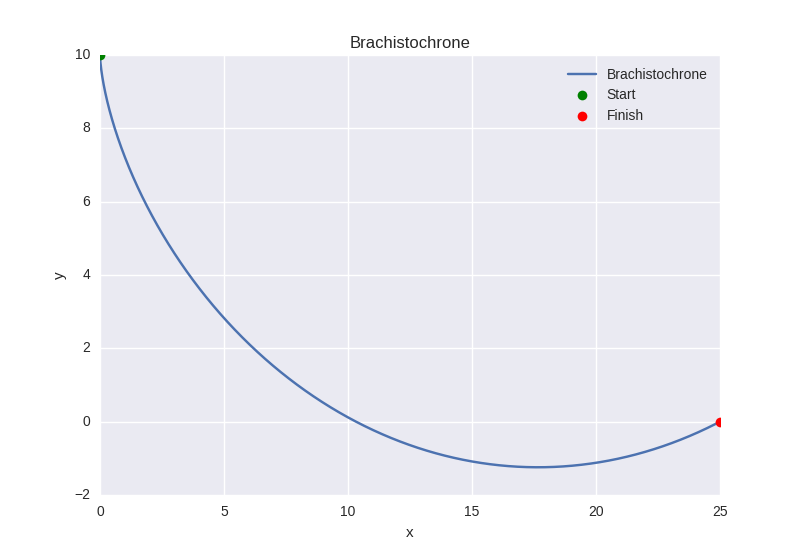
\includegraphics[scale=0.5]{brach.png}
\caption{A brachistochrone going from $(0,10)$ to $(25,0)$}
\end{figure}

We can see that the path of the ball/mass goes below 0, but even though is has to move uphill for the last stretch it is still the fastest route.

\subsection*{e)}
To find the extrema of $y(\theta)$ we are going set its derivatives equal to zero. So

$$
\frac{dy}{d\theta} = -\frac{1}{2}k^2\sin\theta = 0
$$

The solutions are 

$$
\theta = n\pi , \qquad n = 0,1,  \cdots
$$

Given that the slops starts at $\theta = 0$ and is a maximum, it is easy to see that the minimum is at $\theta = \pi$. If we insert this into the definitions of $x$ and $y$ we get that

$$
x(\pi) = \frac{1}{2}k^2(\theta - \sin\theta) = \frac{1}{2}k^2 \pi
$$

$$
y(\pi) = \frac{1}{2}k^2(\cos\pi - 1) = -k^2
$$

This gives us that

$$
y_B = -\frac{2}{\pi}x_B
$$

We can now find the time for a mass to fall to this point. We wish to integrate between $\theta = 0$ and $\pi$. To do this we are going to use a small trick. But first, to make it easier to write I am again going to use that $\frac{1}{2}k^2 = r$

$$
\left(\frac{ds}{d\theta}\right)^2= \left(\frac{dx}{d\theta}\right)^2 + \left(\frac{dx}{d\theta}\right)^2
$$

$$
= r^2((1-\cos\theta)^2 + sin^2\theta) = 2r^2(1-\cos\theta)
$$

$$
\Rightarrow ds = \sqrt{2r^2(1-\cos\theta)}
$$

We remember from earlier that 

$$
v = \sqrt{-2gy} = \sqrt{-2gr(\cos\theta-1)}
$$

We are again going to use that

$$
T = \int dt = \int \frac{ds}{v} = \int_{0}^{\pi} \sqrt{\frac{2r^2(1-\cos\theta)}{-2gr(\cos\theta-1)}} d\theta = \int_{0}^{\pi} \sqrt{\frac{r}{g}} d\theta 
$$
$$
= \pi \sqrt{\frac{r}{g}} =  k\sqrt{\frac{\pi^2}{2g}}
$$

We then find the time if the path was a straight line. We can do this without using any integral. First we find the acceleration felt by the mass

$$
a = -g\cos\theta
$$

We know that the slope is the same all the way, we also know that 

$$
y_B = -\frac{2}{\pi}x_b \Rightarrow \frac{x_B}{y_B} = -\frac{\pi}{2} = \tan\theta 
$$

($\tan\theta$ is defined this way because we are using that the y-axis is at $\theta = 0$). If we use this expression in the acceleration we get

$$
a = -\frac{g}{\sqrt{1+\frac{\pi^2}{4}}}
$$

We now find the total length of the slope

$$
s^2 = x^2 + y^2 = y^2(1+\frac{\pi^2}{4})
$$

We can now use our old friend

$$
s = \frac{1}{2}at^2
$$
$$
\Rightarrow y\sqrt{1+\frac{\pi^2}{4}} = -\frac{1}{2}\frac{gt^2}{\sqrt{1+\frac{\pi^2}{4}}}
$$
$$
\Rightarrow t = T = \sqrt{\frac{-2y}{g}\left(1 + \frac{\pi^2}{4}\right)}
$$

We can so use that $y = y_B = \frac{1}{2}k^2(\cos\pi - 1) = -k^2$

$$
T = k\sqrt{\frac{\pi^2}{2g} + \frac{2}{g}}
$$

If we compare this with the time for the brachistochrone, we can see that the brachistochrone is faster by a time 

$$
\Delta t = -k\sqrt{\frac{2}{g}}
$$

As we expected.
\end{document}


